% Trabalho 4 — Testes de desempenho: Link Extractor
% Compilar: pdflatex apresentacao-trabalho4.tex (2x)
\documentclass[aspectratio=169,11pt]{beamer}

\usetheme{Madrid}
\usecolortheme{default}
\usefonttheme{professionalfonts}

\usepackage[brazil]{babel}
\usepackage[T1]{fontenc}
\usepackage[utf8]{inputenc}
\usepackage{booktabs}
\usepackage{graphicx}
\usepackage{listings}
\usepackage{tikz}
\usetikzlibrary{positioning,arrows.meta}
\usepackage{hyperref}
\usepackage{amssymb}

\hypersetup{colorlinks=true,linkcolor=blue,urlcolor=blue}

\lstset{
  basicstyle=\ttfamily\footnotesize,
  breaklines=true,
  frame=single,
  backgroundcolor=\color{black!5},
  columns=fullflexible,
}

\title{Testes de Desempenho com a Aplicação\\Link Extractor}
\subtitle{Trabalho 4 --- Sistemas Distribuídos}
\author{Francisco Ricardo Teles \\{\small 2317443}\\[0.4em]
  Silvio Bruno Do Nascimento Lima \\{\small 2313199}}
\institute{Sistemas Distribuídos}
\date{30 de outubro de 2026}

\begin{document}

\begin{frame}
  \titlepage
\end{frame}

\begin{frame}{Agenda}
  \tableofcontents
\end{frame}

\section{Aplicação Link Extractor}

\begin{frame}{Objetivo do trabalho}
  \begin{block}{Enunciado}
    Avaliar desempenho das versões \textbf{Python} e \textbf{Ruby} do serviço de
    extração de links, com e sem \textbf{cache Redis}, usando ferramenta de carga
    configurável por script (\textbf{Locust}).
  \end{block}
  \begin{itemize}
    \item Cada usuário virtual realiza \textbf{10 invocações} com \textbf{URLs distintas}
    \item Variar: nº de usuários, linguagem da API e uso do cache
    \item Registrar média, mediana e percentis do tempo de resposta
  \end{itemize}
\end{frame}

\begin{frame}{Arquitetura}
  \centering
  \begin{tikzpicture}[
    node distance=0.85cm and 1.1cm,
    box/.style={draw, rounded corners, minimum width=2.4cm, minimum height=0.8cm, align=center, font=\small},
    arr/.style={-{Stealth[length=2.5mm]}, thick}
  ]
    \node[box, fill=blue!12] (locust) {Locust};
    \node[box, fill=orange!18, right=of locust] (web) {Web PHP};
    \node[box, fill=green!15, right=of web] (api) {API\\Python / Ruby};
    \node[box, fill=red!12, below=of api] (redis) {Redis};
    \node[box, fill=gray!15, above right=0.3cm and 0.8cm of api] (net) {Páginas\\externas};

    \draw[arr] (locust) -- node[above,font=\scriptsize]{/api/...} (api);
    \draw[arr] (locust) -- node[below,font=\scriptsize]{opcional} (web);
    \draw[arr] (web) -- (api);
    \draw[arr] (api) -- node[right,font=\scriptsize]{HIT/MISS} (redis);
    \draw[arr] (api) -- (net);
  \end{tikzpicture}

  \vspace{0.4em}
  {\small Base: tutorial Play-with-Docker / repositório \texttt{linkextractor} (steps 4--6).}
\end{frame}

\begin{frame}{Versões sob teste}
  \small
  \begin{tabular}{@{}lll@{}}
    \toprule
    Cenário & API & Cache \\
    \midrule
    \texttt{python-com-cache} & Flask (step5) :5000 & Redis \\
    \texttt{python-sem-cache} & Flask (step4) :5000 & --- \\
    \texttt{ruby-com-cache} & Sinatra (step6) :4567 & Redis \\
    \texttt{ruby-sem-cache} & Sinatra (sem Redis) :4567 & --- \\
    \bottomrule
  \end{tabular}
  \vspace{0.6em}

  Com cache: se a URL já foi extraída, a API devolve JSON do Redis sem baixar a página novamente.
\end{frame}

\section{Ferramenta e script Locust}

\begin{frame}{Ferramenta: Locust}
  \begin{itemize}
    \item Open-source, script em Python, UI web e modo \emph{headless}
    \item Usuários virtuais = classe \texttt{HttpUser} com tarefas (\texttt{@task})
    \item Métricas: RPS, tempo médio, mediana, percentis (P95), falhas
    \item Imagem Docker: \texttt{locustio/locust:2.29.0}
    \item Alvo: serviço de extração (\texttt{http://api:5000} ou \texttt{:4567})
  \end{itemize}
\end{frame}

\begin{frame}[fragile]{Script do usuário virtual}
  \begin{lstlisting}[language=Python,basicstyle=\ttfamily\tiny]
URLS = [  # 10 URLs distintas
  "http://example.com/", "https://example.org/", ... ]

class LinkExtractorUser(HttpUser):
    wait_time = between(0.5, 1.5)

    @task
    def extrair_dez_urls(self):
        for i, url in enumerate(URLS, start=1):
            self.client.get(
                f"/api/{url}",
                name=f"extract_{i:02d}",
                timeout=120,
            )
  \end{lstlisting}
  \vspace{0.3em}
  {\small Arquivo: \texttt{desempenho/locust/locustfile.py} --- 10 GETs sequenciais por tarefa.}
\end{frame}

\begin{frame}{URLs utilizadas nas 10 invocações}
  \scriptsize
  \begin{enumerate}
    \item \texttt{http://example.com/}
    \item \texttt{https://example.org/}
    \item \texttt{https://www.iana.org/domains/reserved}
    \item \texttt{https://httpbin.org/html}
    \item \texttt{https://www.w3.org/TR/html401/intro/intro.html}
    \item \texttt{https://info.cern.ch/}
    \item \texttt{https://www.rfc-editor.org/rfc/rfc2616}
    \item \texttt{https://books.toscrape.com/}
    \item \texttt{https://quotes.toscrape.com/}
    \item \texttt{https://webscraper.io/test-sites/e-commerce/static}
  \end{enumerate}
\end{frame}

\section{Cenários de teste}

\begin{frame}{Matriz experimental}
  \begin{columns}[T]
    \column{0.52\textwidth}
    \textbf{Fatores}
    \begin{itemize}
      \item Usuários: \textbf{5}, \textbf{15}, \textbf{40}
      \item Linguagem: Python / Ruby
      \item Cache: com / sem
    \end{itemize}
    Total: $3 \times 2 \times 2 = 12$ execuções.
    \column{0.46\textwidth}
    \textbf{Parâmetros Locust}
    \begin{itemize}
      \item Duração: 90\,s
      \item Spawn: $\min(\text{users}, 10)$
      \item Wait: 0,5--1,5\,s
      \item Saída: CSV + \texttt{manifest.json}
    \end{itemize}
  \end{columns}
  \vspace{0.5em}
  \begin{block}{Ambiente}
    Windows 10, Docker Desktop, 16\,GB RAM; Compose em \texttt{desempenho/compose/}.
  \end{block}
\end{frame}

\begin{frame}[fragile]{Automação}
  \begin{lstlisting}[language=bash,basicstyle=\ttfamily\tiny]
# Subir um cenario
.\scripts\set_cenario.ps1 -Cenario python-com-cache

# Um teste
.\scripts\run_locust_headless.ps1 -Cenario ruby-sem-cache -Usuarios 15

# Matriz completa + graficos
.\scripts\run_matriz_testes.ps1
  \end{lstlisting}
\end{frame}

\section{Resultados}

\begin{frame}{Resultados --- 15 usuários virtuais}
  \scriptsize
  \centering
  \begin{tabular}{@{}lrrrr@{}}
    \toprule
    Cenário & RPS & Média (ms) & Mediana (ms) & P95 (ms) \\
    \midrule
    python-com-cache  & 9,6  & 720  & 634  & 1129 \\
    python-sem-cache  & 7,1  & 1310 & 1153 & 2053 \\
    ruby-com-cache    & 8,2  & 917  & 807  & 1437 \\
    ruby-sem-cache    & 6,1  & 1572 & 1383 & 2464 \\
    \bottomrule
  \end{tabular}
  \vspace{0.5em}

  {\small Fonte: agregado Locust (90\,s), \texttt{resultados/manifest.json}.}
\end{frame}

\begin{frame}{Gráficos --- RPS e latência média}
  \centering
  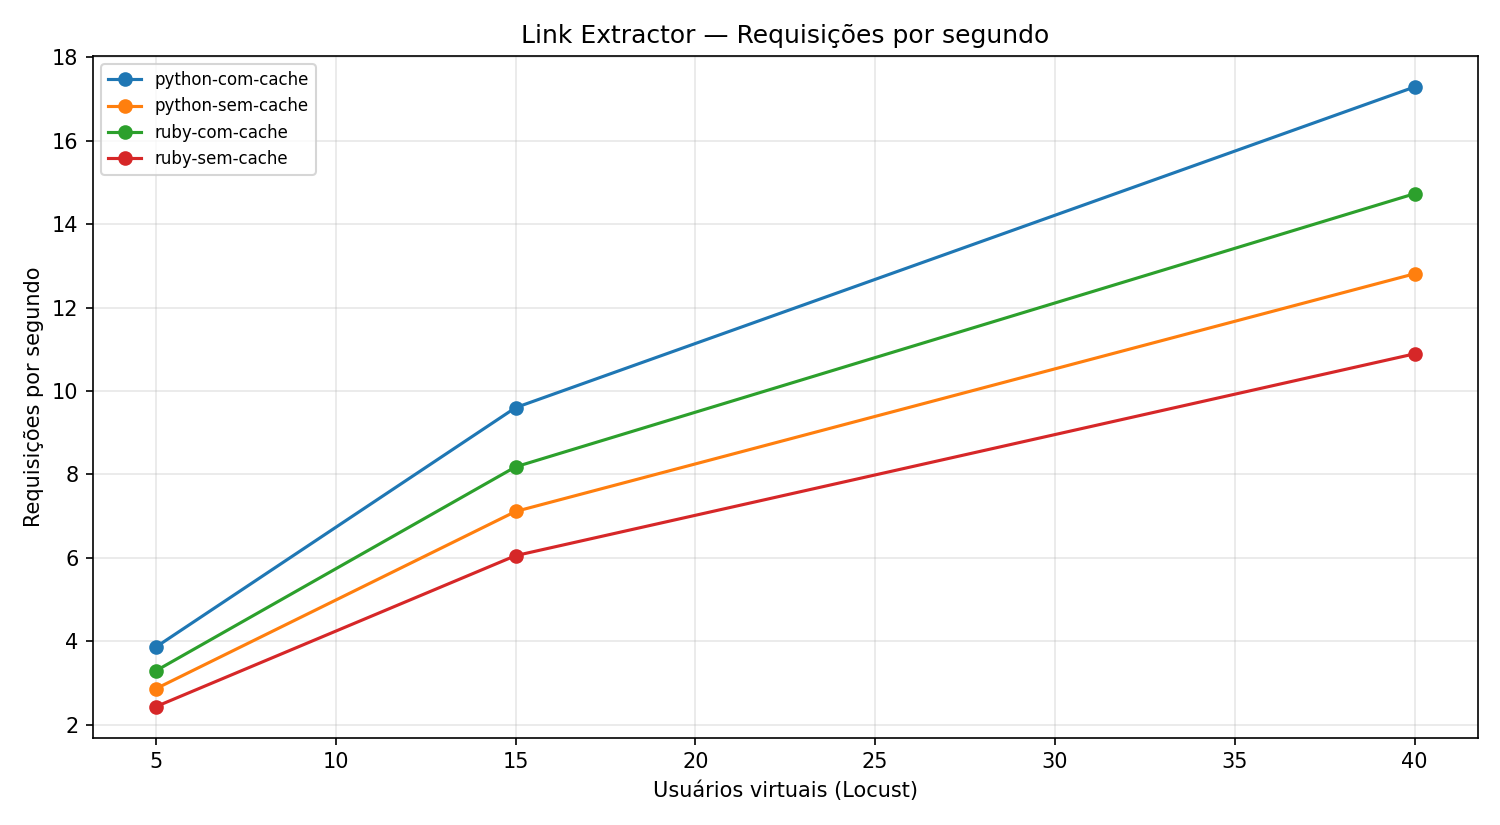
\includegraphics[width=0.48\textwidth]{desempenho/graficos/rps_por_usuarios.png}\hfill
  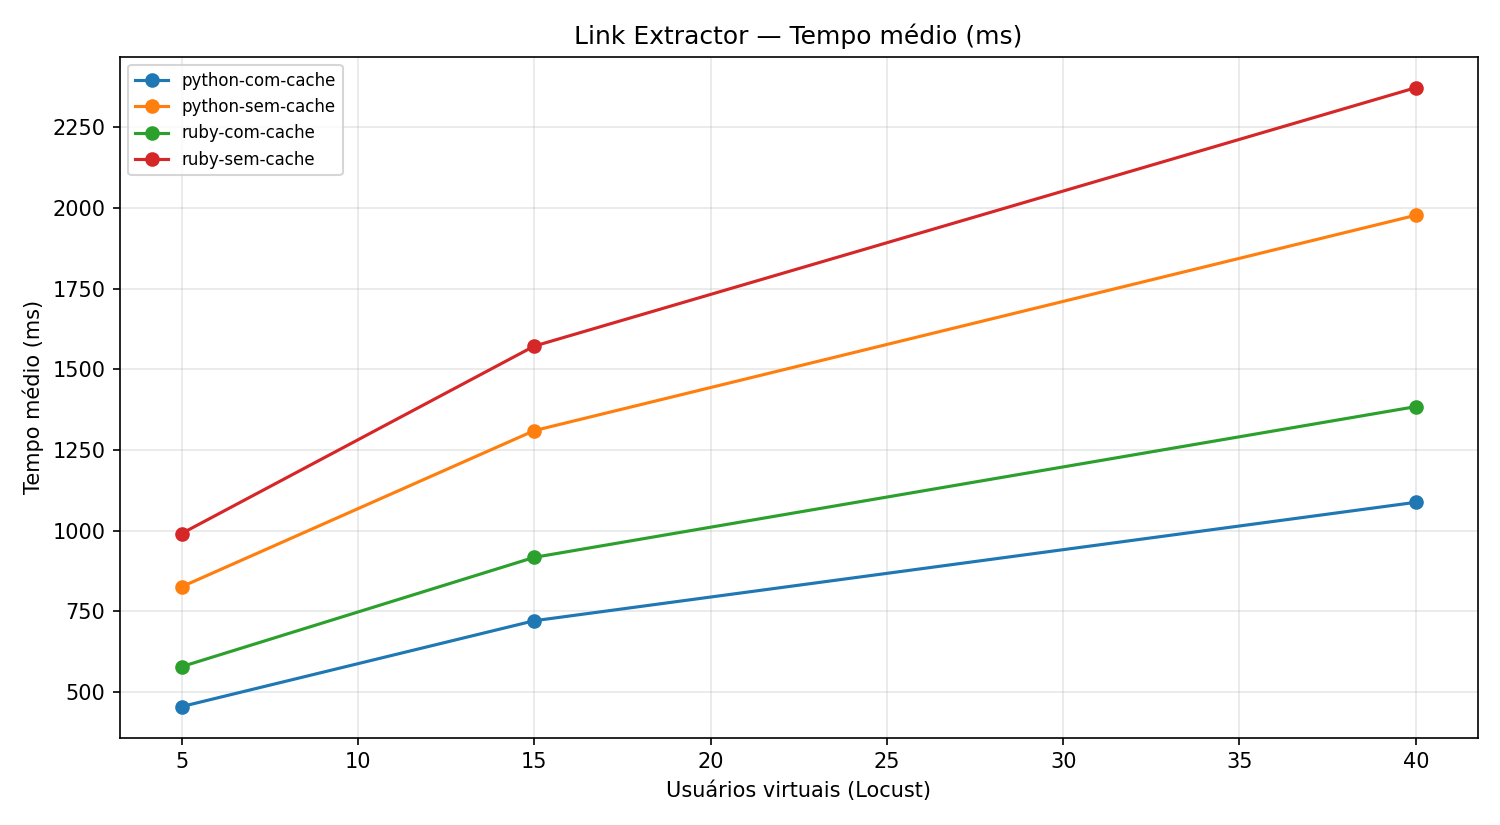
\includegraphics[width=0.48\textwidth]{desempenho/graficos/avg_por_usuarios.png}
\end{frame}

\begin{frame}{Gráficos --- P95 e mediana}
  \centering
  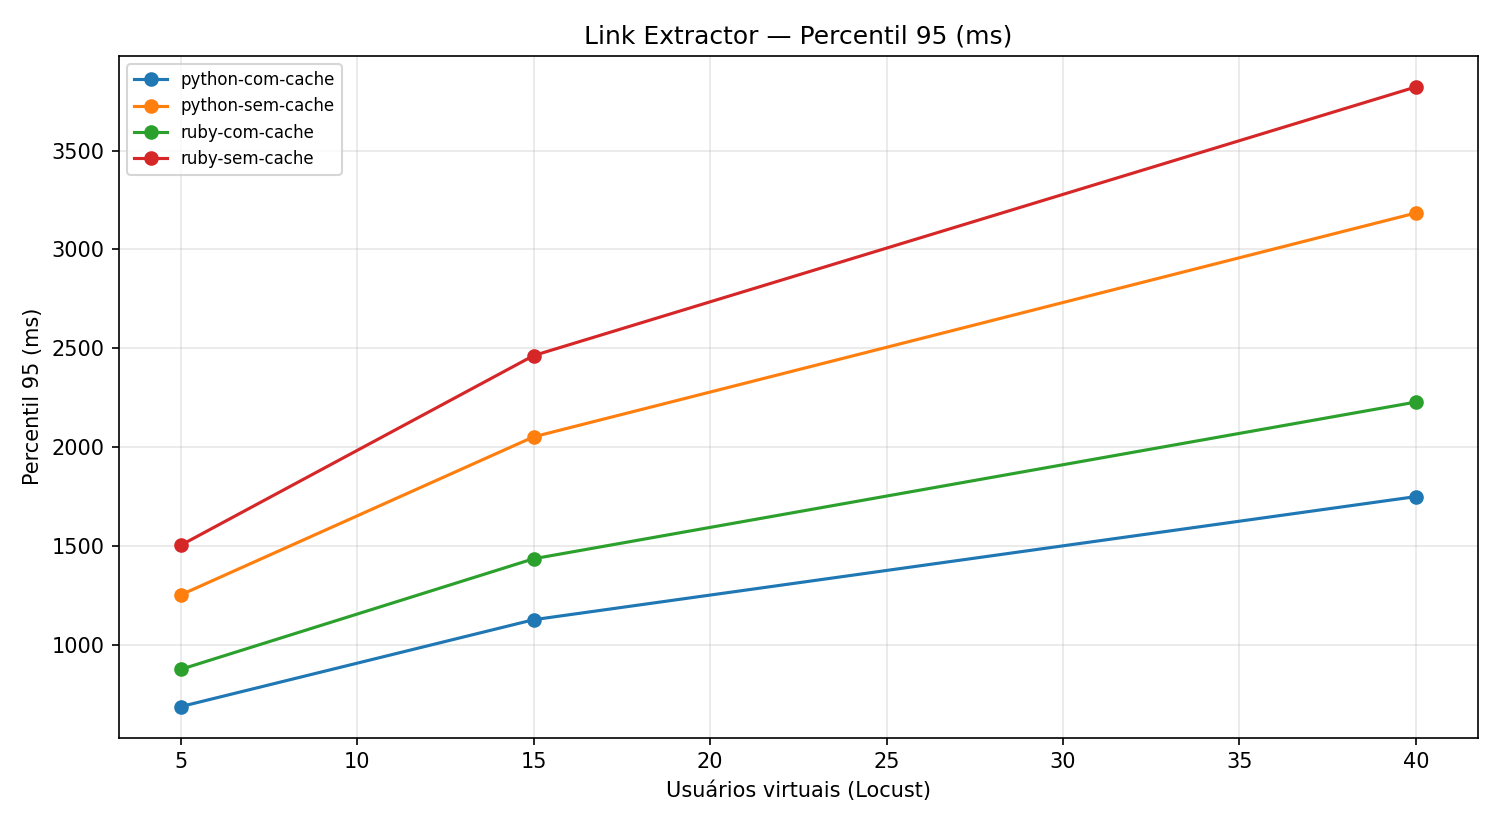
\includegraphics[width=0.48\textwidth]{desempenho/graficos/p95_por_usuarios.png}\hfill
  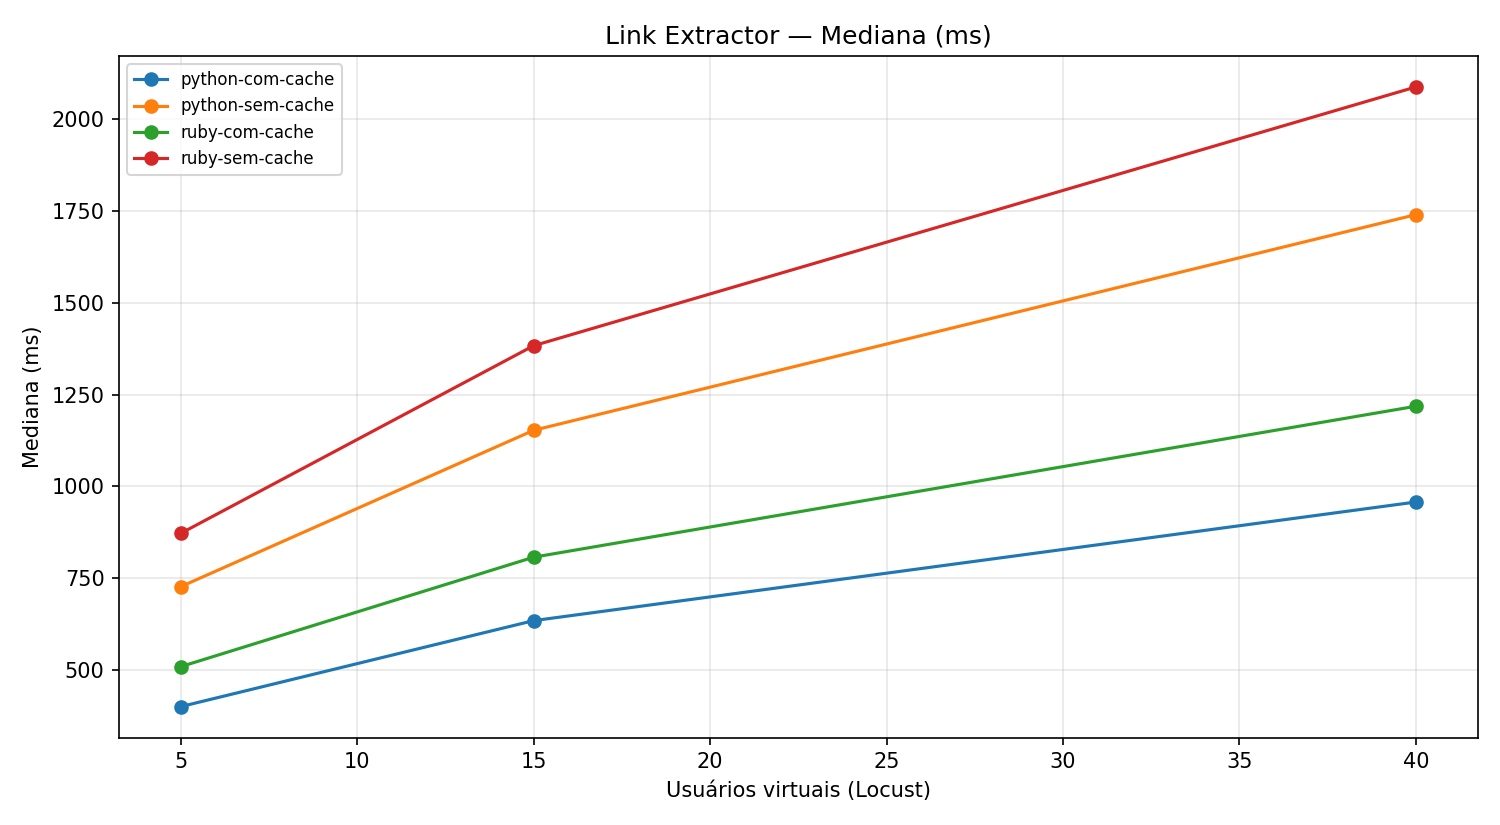
\includegraphics[width=0.48\textwidth]{desempenho/graficos/median_por_usuarios.png}
\end{frame}

\begin{frame}{Comparativo --- 15 e 40 usuários}
  \centering
  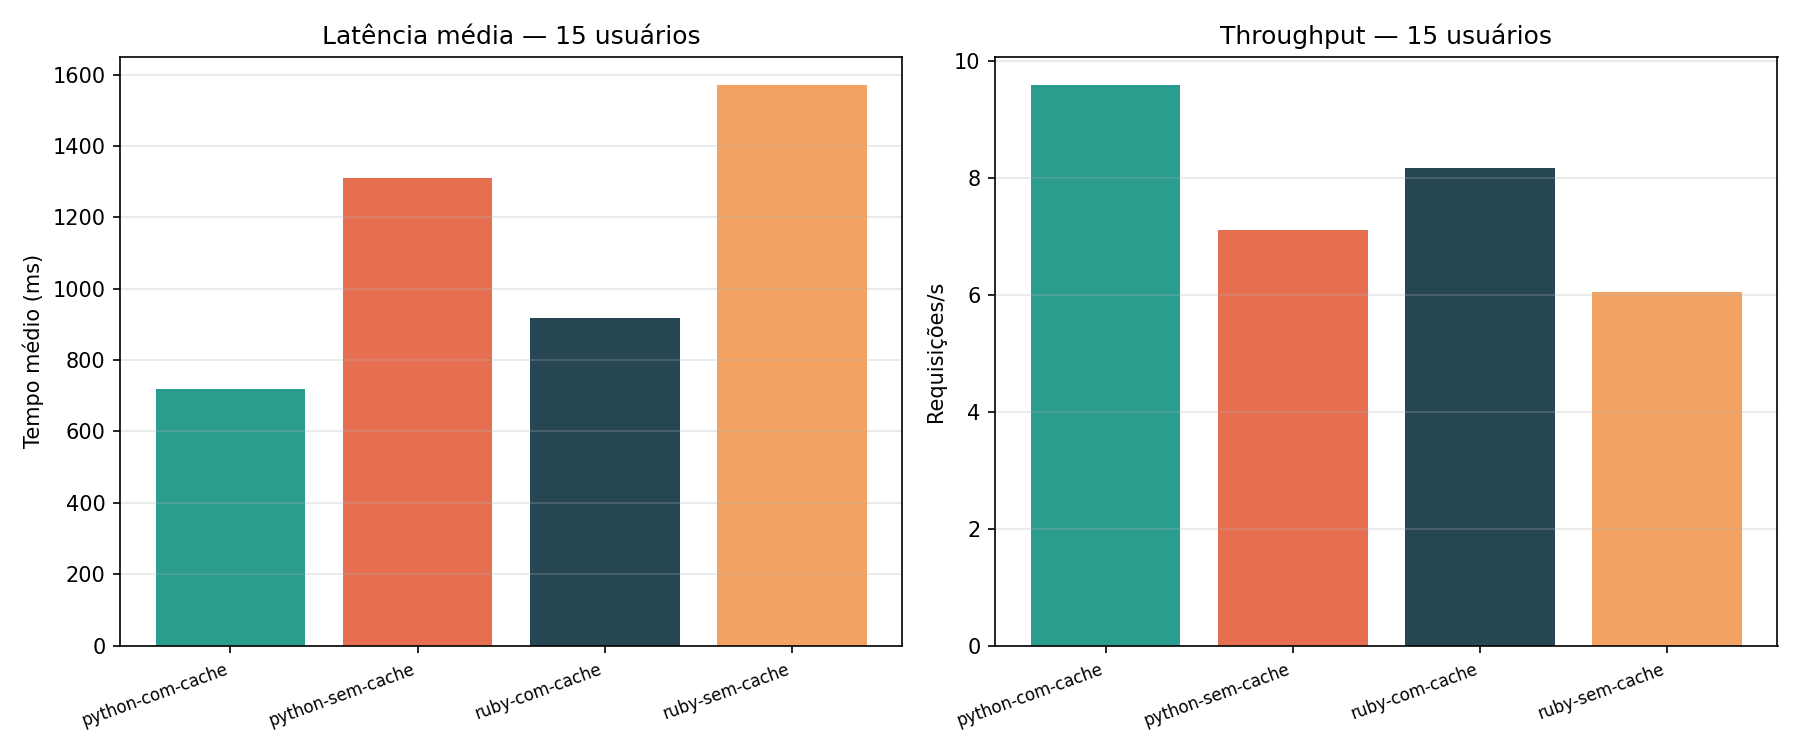
\includegraphics[width=0.48\textwidth]{desempenho/graficos/comparativo_15_usuarios.png}\hfill
  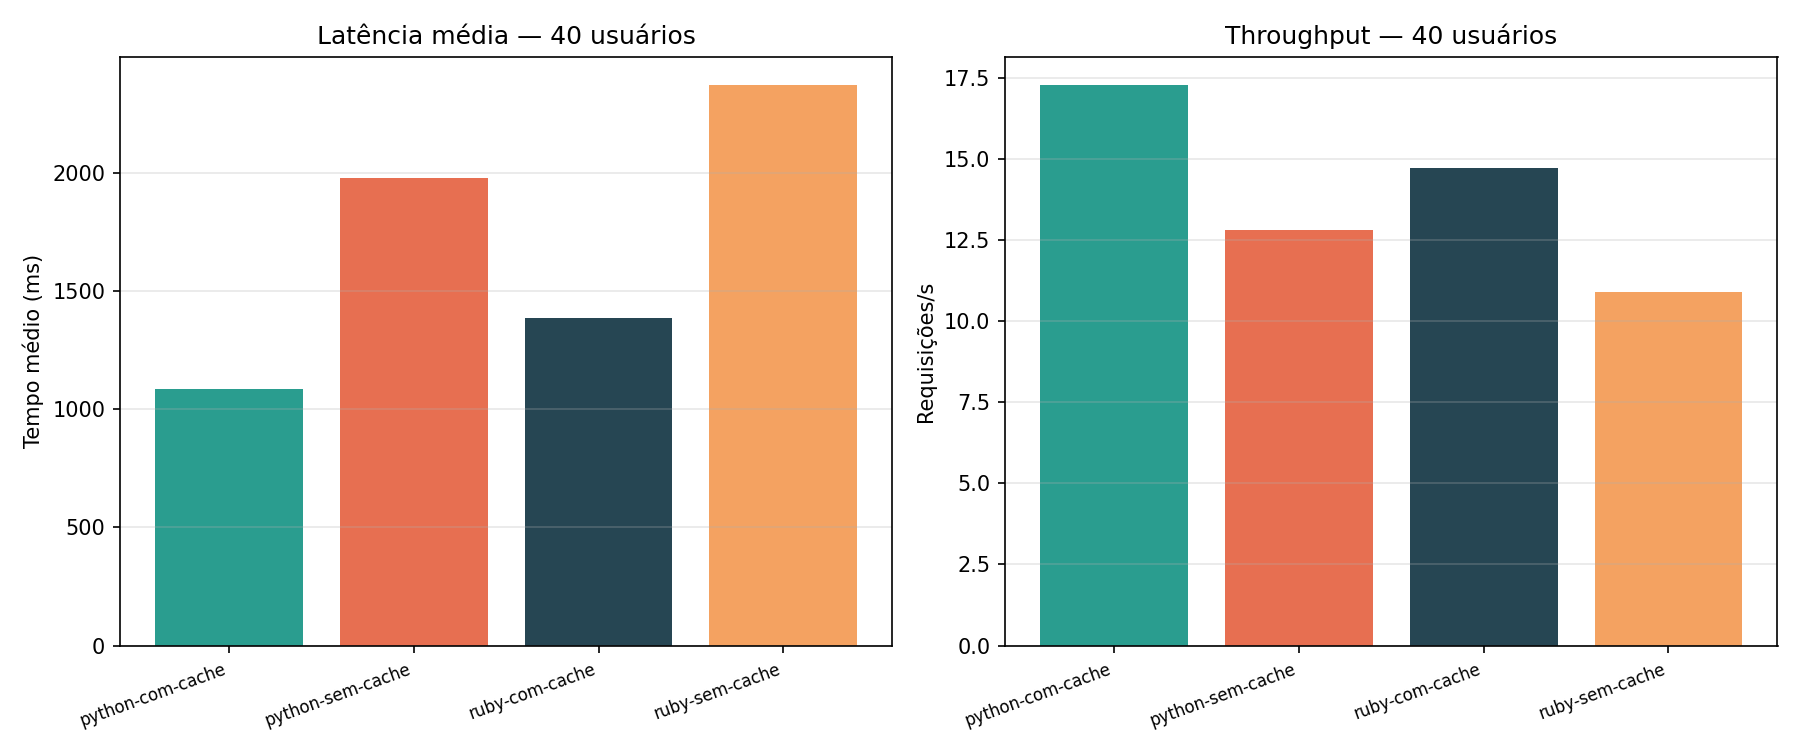
\includegraphics[width=0.48\textwidth]{desempenho/graficos/comparativo_40_usuarios.png}
\end{frame}

\begin{frame}{Interpretação}
  \begin{itemize}
    \item \textbf{Cache Redis} reduz latência $\approx$45\% (Python: 1310\,ms $\rightarrow$ 720\,ms com 15 usuários) e eleva RPS.
    \item \textbf{Python} superou \textbf{Ruby} nestas condições (RPS e latência), com e sem cache.
    \item Sem cache, cada uma das 10 URLs força download + parse HTML --- custo dominante.
    \item Com cache, após o primeiro HIT compartilhado entre usuários, o Redis evita I/O externo.
    \item Em 40 usuários, o P95 sobe em todos os cenários; o ganho relativo do cache permanece.
  \end{itemize}
\end{frame}

\section{Conclusão}

\begin{frame}{Entregáveis}
  \begin{itemize}
    \item[\checkmark] Equipe e matrículas na capa
    \item[\checkmark] Locust descrito + script do usuário (10 URLs)
    \item[\checkmark] Cenários: usuários $\times$ Python/Ruby $\times$ com/sem cache
    \item[\checkmark] Gráficos (RPS, média, mediana, P95) e tabela de métricas
    \item[\checkmark] Código em \texttt{Trabalho4/desempenho/}
  \end{itemize}
\end{frame}

\begin{frame}{Conclusão}
  \begin{itemize}
    \item O Link Extractor em microsserviços permite trocar a API (Python $\leftrightarrow$ Ruby) e medir o impacto do cache de forma isolada.
    \item O Locust modelou o comportamento pedido (10 URLs distintas por usuário) e gerou métricas comparáveis.
    \item O cache Redis é o fator de maior impacto; a escolha da linguagem tem efeito secundário, porém mensurável.
  \end{itemize}
  \vspace{1em}
  \centering
  \Large Obrigado --- perguntas?
\end{frame}

\end{document}
